% QuAM-GDN: ACL / ARR submission draft (short version of paper_journal/main.tex).
% Compile: pdflatex main; bibtex main; pdflatex main; pdflatex main   (or upload the folder to Overleaf)
% Numbers: reports/final_numbers.json, reports/sig_gdn/*.json, reports/memory_significance.json,
% reports/ablation.json, reports/final_analysis.json (see paper_journal/main.tex for the scripts).
\documentclass[11pt]{article}
\usepackage[review]{acl}          % remove "review" for the camera-ready version
\usepackage{times}
\usepackage{latexsym}
\usepackage[T1]{fontenc}
\usepackage[utf8]{inputenc}
\usepackage{microtype}
\usepackage{inconsolata}
\usepackage{graphicx}
\usepackage{booktabs}
\usepackage{multirow}
\usepackage{amsmath,amssymb}
\usepackage{bm}
\usepackage{xcolor}

\newcommand{\pmstd}[2]{#1{\scriptsize$\pm$#2}}
\newcommand{\quam}{QuAM-GDN}

\title{Aspect-Prompted Delta-Rule Memory for Zero-Shot Aspect-Based\\
Sentiment Analysis of Code-Mixed Bangla E-Commerce Reviews}

% Anonymous for review. Fill in for the camera-ready version.
\author{First Author \\ Daffodil International University \\ \texttt{email@domain} \And
        Second Author (Supervisor) \\ Daffodil International University \\ \texttt{email@domain}}

\begin{document}
\maketitle

\begin{abstract}
Aspect-based sentiment analysis (ABSA) of Bangladeshi e-commerce reviews must handle Bangla, romanised
Bangla (Banglish) and English, often mixed, and product categories whose aspect inventories keep
changing. We present \quam{}, which writes all candidate aspect names of a product category into the
input of a fine-tuned multilingual encoder, represents each aspect by the mean of the encoder states
over its own name, and uses this contextual name both in a per-aspect scorer and as the query to a
bidirectional Gated DeltaNet memory, a delta-rule recurrent memory that we adapt to be read by aspect
names. Against fine-tuned BanglaBERT and XLM-R trained under identical conditions, \quam{} improves
strict aspect--sentiment pair F1 on EComReviews-BD by 10.7 points on the standard split (72.7), 9.3 on
a leakage-free split (71.2) and 18.4 on unseen product categories (57.3), all $p<0.001$, and reaches
36.7 pair F1 on unseen aspect names where the classifiers reach at most 3.1. The aspect prompt is the
largest gain; the delta-rule memory, unlike an xLSTM memory, significantly improves unseen (+2.0) and
rare aspect names. We release a leakage-free and a zero-shot split.
\end{abstract}

% =========================================================================
\section{Introduction}

Daraz and other Bangladeshi marketplaces collect short product reviews in Bangla script, Banglish,
English, or a mixture; such code-mixed text is hard for sentiment models \citep{patwa2020sentimix}.
Sellers need aspect-level sentiment \citep{pontiki2014semeval,zhang2023absasurvey}: which of a
category's aspects (price, delivery, battery, \dots) a review mentions, and with which polarity. The
inventory is open: new categories bring aspect names a classifier with one output per known aspect
cannot score. And compute is scarce; all our experiments run on a 4\,GB laptop GPU.

Pairing the review with each aspect \citep{sun2019auxiliary} handles any name at one encoder pass per
aspect. Multi-aspect models put all aspects into one input \citep{wu2020tmm} or read one encoding with
aspect-specific readouts \citep{xia2026dabs}, but assume given, known aspects in English. Zero-shot
aspect category sentiment analysis has been studied with generation models and LLMs, again for English
\citep{liu2021acsagen,ventirozos2025zeroshotacsa}.

\quam{} writes the category and all its candidate aspect names into the first input segment, fine-tunes
the encoder, and pools each aspect from its own name span. The pooled name scores the aspect directly
and queries a bidirectional \emph{Gated DeltaNet} memory \citep{yang2025gdn}, whose delta rule
overwrites the association stored under a key instead of adding to it. Our contributions:
(1) \quam{}, which detects and classifies all candidate aspects in one pass and handles unseen names
without new parameters; to our knowledge the first delta-rule memory for ABSA and the first aspect-name
read-out of such a memory; (2) a controlled comparison with fine-tuned BanglaBERT and XLM-R, in which
\quam{} improves pair F1 by 9.3--29.9 points on all splits; (3) ablations showing that the aspect prompt
is the main gain and that the delta-rule memory, unlike an xLSTM memory, significantly helps unseen and
rare aspect names; (4) a leakage-free split (11.5\% of standard test reviews occur in training) and a
zero-shot category split.

% =========================================================================
\section{Related Work}

\paragraph{ABSA.} Memory networks \citep{tang2016memnet} and aspect-attention LSTMs \citep{wang2016atae}
were followed by sentence-pair BERT models \citep{sun2019auxiliary}. Joint models predict all
categories at once \citep{schmitt2018joint,hu2019can}. TMM \citep{wu2020tmm} appends all categories with
marker tokens and classifies each from its marker, without detection and for eight fixed English
categories; DABS \citep{xia2026dabs} reads given aspect spans from one encoding. We add detection,
span-pooled name queries, a recurrent memory, and evaluation on unseen aspects. \citet{liu2021acsagen}
and \citet{ventirozos2025zeroshotacsa} study zero-shot ACSA in English, and \citet{fehle2026crosslingual}
cross-lingual ABSA; LLMs still trail small in-domain models on ABSA \citep{zhang2024llmsentiment}.

\paragraph{Linear recurrent memories.} Linear attention and fast weights store key--value outer
products in a matrix \citep{katharopoulos2020transformers,schlag2021fastweights}; the mLSTM of xLSTM adds
gates to this additive update \citep{beck2024xlstm,beck2025xlstm7b}. The delta rule
\citep{schlag2021fastweights,yang2024deltanet} first removes the stored value, and Gated DeltaNet
\citep{yang2025gdn} adds a forget gate; it was proposed for causal language modelling. xLSTM ABSA work
lets the aspect gate the memory \emph{writes} \citep{lawan2025afmat,lawan2025gatemabsa}, one pass per
aspect; our aspects \emph{read} a finished memory.

\paragraph{Bangla.} Bangla ABSA datasets were small \citep{rahman2018banglaabsa,masum2020banabsa} until
EComReviews-BD \citep{haque2026ecomreviews} and BABSA \citep{rohman2025babsa}. BanglaBERT
\citep{bhattacharjee2022banglabert} and XLM-R \citep{conneau2020xlmr} are the usual encoders.

% =========================================================================
\begin{figure*}[t]
\centering
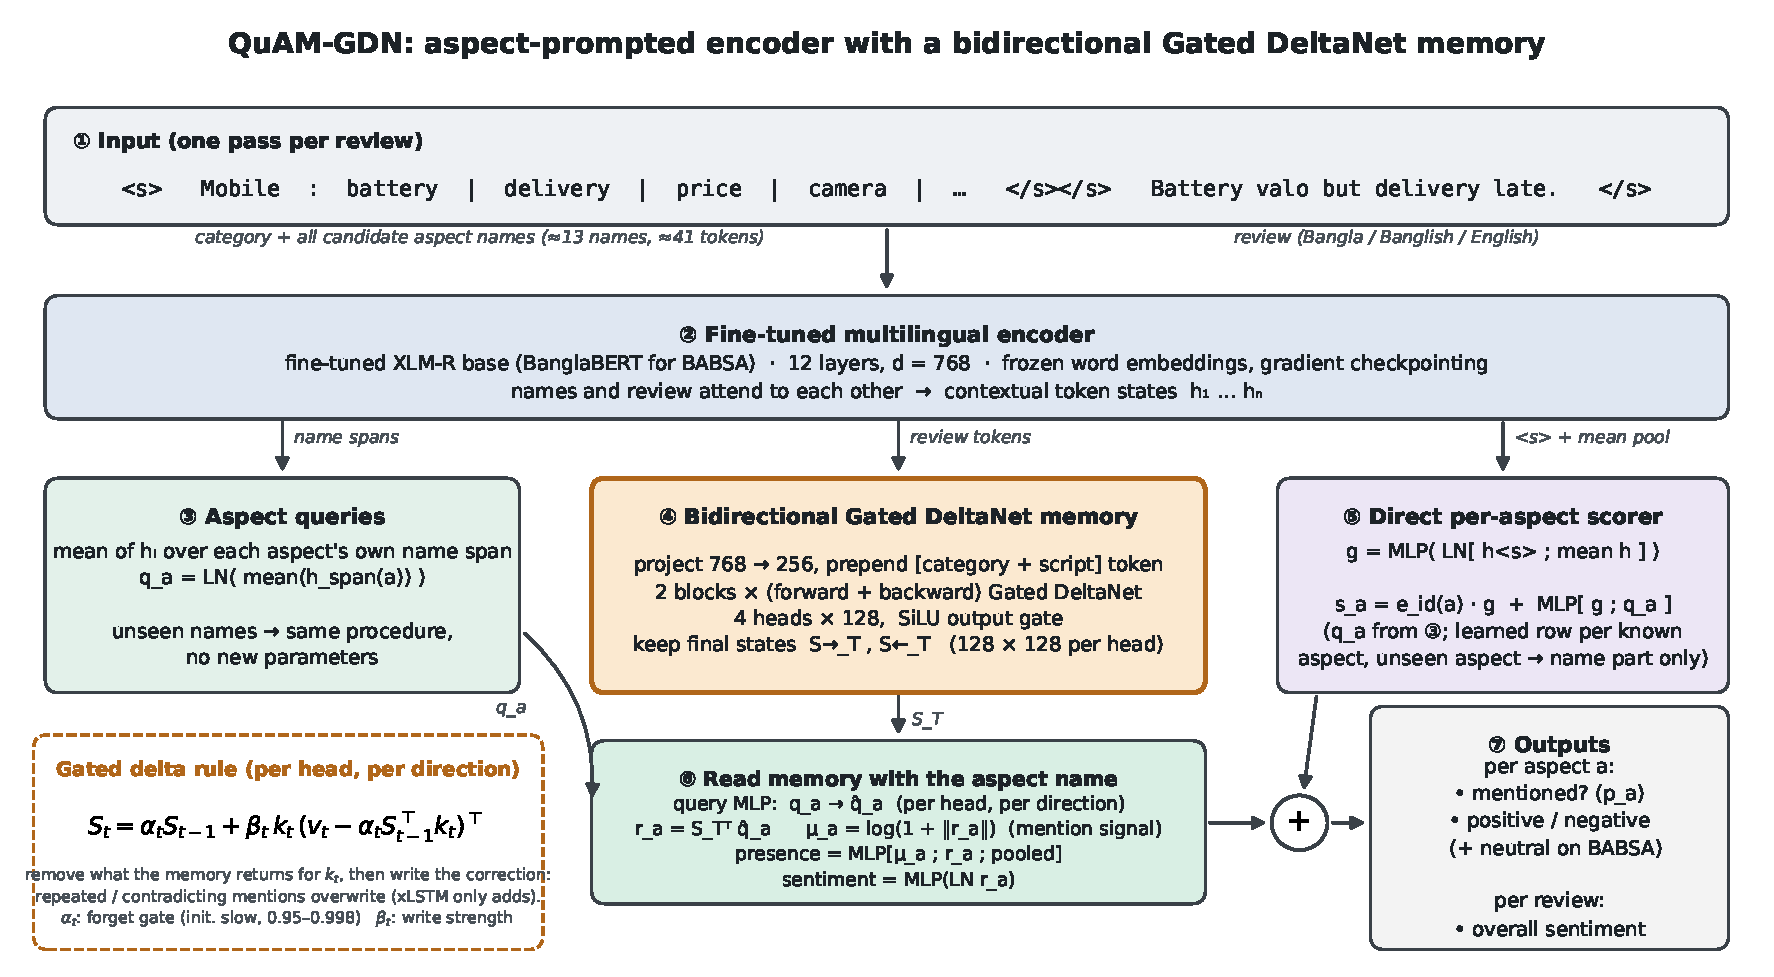
\includegraphics[width=\textwidth]{figures/architecture.pdf}
\caption{\quam{}. Category and candidate aspect names are written into the input of a fine-tuned encoder; each aspect
query is the mean over its name span, reads the final state of a bidirectional Gated DeltaNet, and is also scored
directly; both scores are added.}
\label{fig:arch}
\end{figure*}

\section{Method}

\paragraph{Aspect-prompted encoding.} Figure~\ref{fig:arch} shows the model. A review $x$ of category $c$ with aspects $\mathcal{A}_c$ (13 on
average) is encoded once as \texttt{<s>} $c$ \texttt{:} $a_1$ \texttt{|} \dots \texttt{|} $a_{|\mathcal{A}_c|}$
\texttt{</s></s>} $x$ \texttt{</s>}. The encoder is fine-tuned (lr $2\times10^{-5}$, frozen word
embeddings, gradient checkpointing). Each aspect query is the layer-normalised mean of the final states
$\mathbf{h}_i$ over its name span $\mathcal{S}_a$:
$\mathbf{q}_a=\mathrm{LN}(|\mathcal{S}_a|^{-1}\sum_{i\in\mathcal{S}_a}\mathbf{h}_i)$. Unseen names are
handled like known ones.

\paragraph{Bidirectional Gated DeltaNet.} The review states, projected to $d{=}256$ and preceded by a
category-and-script prefix token, pass through two pre-norm blocks; each runs a Gated DeltaNet cell in
both directions (4 heads of size 128, SiLU output gate). Per head, with L2-normalised keys, write
strength $\beta_t\in(0,1)$ and decay $\alpha_t\in(0,1)$,
\begin{equation}
\mathbf{S}_t = \alpha_t\mathbf{S}_{t-1} + \beta_t\,\mathbf{k}_t\big(\mathbf{v}_t - \alpha_t\mathbf{S}_{t-1}^\top\mathbf{k}_t\big)^\top ,
\end{equation}
i.e.\ only the correction between the new value and what the memory returns for $\mathbf{k}_t$ is
written, so repeated or contradicting mentions overwrite rather than accumulate (the mLSTM adds
$i_t\mathbf{v}_t\mathbf{k}_t^\top$). We adapt the published model by running it bidirectionally,
reading only the final states with external aspect queries, initialising the decay bias to 3--6 (slow
forgetting), and masking padding ($\beta{=}0,\alpha{=}1$). We implement the chunkwise WY form in
PyTorch (no pretrained weights; error vs.\ the recurrent form $5\times10^{-7}$).

\paragraph{Read-out and scoring.} An MLP maps $\mathbf{q}_a$ to one normalised query $\hat{\mathbf{q}}$
per head and direction; the read is $\mathbf{r}_a=\mathbf{S}_T^\top\hat{\mathbf{q}}_a$ with mention
signal $\mu_a=\log(1+\|\mathbf{r}_a\|)$. Presence and sentiment logits from the read are added to a
direct scorer $s_a=\mathbf{e}_{\mathrm{id}(a)}^\top\mathbf{g}+\mathrm{MLP}([\mathbf{g};\mathbf{q}_a])$ over
pooled encoder states $\mathbf{g}$, with a zero-initialised row per known aspect (unseen names: zero
row; ids dropped with probability 0.2 in training). Overall sentiment aggregates aspect sentiments by
learned importance plus a memory read with the query ``overall opinion''. Losses: presence BCE, sentiment
CE, $0.5\times$ overall CE.

% =========================================================================
\section{Data and Setup}

\paragraph{EComReviews-BD} \citep{haque2026ecomreviews}: 20,685 Daraz reviews, 19 categories, 74 aspect
names (37\% Bangla, 45\% English, 12\% Banglish, 6\% mixed). We reproduce the official 70/15/15 split;
358 of its 3,103 test texts (11.5\%) also occur in training, so we add a \emph{grouped} split without
cross-split duplicates and a \emph{zero-shot} split whose test set is four unseen categories (2,637
reviews; 956 of 2,750 mentions have one of 18 aspect names unseen in training).
\paragraph{BABSA} \citep{rohman2025babsa}: 14,099 Bangla texts, 16,968 (text, term) pairs, three
polarities; grouped 70/15/15 split. Candidate terms are the gold terms plus three sampled negatives, in
shuffled order.
\paragraph{Metrics.} Strict pair F1 (micro; detected \emph{and} correct polarity), detection macro-F1
over aspect names, polarity accuracy, overall macro-F1; BABSA: macro-F1 over gold terms. Every system's
presence threshold is tuned on validation.
\paragraph{Baselines and training.} Fine-tuned BanglaBERT and XLM-R on (category, review) with one
output row per aspect, same losses, lr, schedule, epochs ($\leq$10, patience 3) and threshold selection.
Three seeds unless marked; paired bootstrap over test reviews (10,000 samples). A run of \quam{} takes
35--60 min on an RTX 2050 (2.9\,GB peak).

% =========================================================================
\section{Results}

\begin{table*}[t]
\centering\footnotesize
\setlength{\tabcolsep}{4pt}
\begin{tabular}{llcccccc}
\toprule
split & model & pair P & pair R & \textbf{pair F1} & det.\ mF1 & pol.\ acc & overall F1 \\
\midrule
\multirow{5}{*}{official}
 & BanglaBERT, reported \citep{haque2026ecomreviews} & 31.8 & 77.1 & 45.0 & -- & -- & -- \\
 & BanglaBERT, fine-tuned & \pmstd{62.4}{1.9} & \pmstd{54.0}{1.1} & \pmstd{57.9}{0.3} & \pmstd{15.4}{0.5} & \pmstd{89.4}{0.4} & \pmstd{78.4}{0.7} \\
 & XLM-R, fine-tuned$^1$ & 67.7 & 57.3 & 62.1 & 17.2 & 89.2 & 78.1 \\
 & XLM-R, frozen + MLP & \pmstd{60.4}{1.6} & \pmstd{56.8}{1.3} & \pmstd{58.6}{0.4} & \pmstd{35.4}{0.9} & \pmstd{85.8}{0.3} & \pmstd{67.5}{0.1} \\
 & \textbf{\quam{}} & \textbf{\pmstd{72.3}{1.4}} & \textbf{\pmstd{73.1}{0.9}} & \textbf{\pmstd{72.7}{0.3}} & \textbf{\pmstd{61.1}{2.0}} & \textbf{\pmstd{90.5}{0.2}} & \textbf{\pmstd{78.7}{0.4}} \\
\midrule
\multirow{3}{*}{grouped}
 & BanglaBERT, fine-tuned & \pmstd{61.4}{2.5} & \pmstd{54.9}{1.6} & \pmstd{58.0}{0.6} & \pmstd{17.4}{0.6} & \textbf{\pmstd{90.1}{0.1}} & \pmstd{77.5}{0.7} \\
 & XLM-R, fine-tuned$^1$ & 63.9 & 60.1 & 61.9 & 21.3 & 88.8 & 76.2 \\
 & \textbf{\quam{}} & \textbf{\pmstd{70.9}{1.7}} & \textbf{\pmstd{71.6}{1.5}} & \textbf{\pmstd{71.2}{0.4}} & \textbf{\pmstd{60.7}{1.4}} & \pmstd{89.9}{0.2} & \textbf{\pmstd{77.9}{0.2}} \\
\midrule
\multirow{3}{*}{zero-shot}
 & BanglaBERT, fine-tuned & \textbf{\pmstd{70.6}{5.9}} & \pmstd{26.9}{1.4} & \pmstd{38.9}{0.7} & \pmstd{13.3}{1.0} & \pmstd{74.4}{0.9} & \pmstd{63.3}{0.6} \\
 & XLM-R, fine-tuned$^1$ & 21.0 & 39.4 & 27.4 & 21.4 & 72.1 & 63.0 \\
 & \textbf{\quam{}} & \pmstd{52.8}{6.1} & \textbf{\pmstd{63.3}{3.8}} & \textbf{\pmstd{57.3}{1.9}} & \textbf{\pmstd{56.8}{1.2}} & \textbf{\pmstd{87.7}{0.3}} & \textbf{\pmstd{64.0}{1.1}} \\
\bottomrule
\end{tabular}
\caption{EComReviews-BD test results (mean$\pm$std over three seeds, $^1$one seed). Bootstrap
differences in pair F1, \quam{} vs.\ BanglaBERT / XLM-R: official $+14.8$ / $+10.7$, grouped $+13.2$ /
$+9.3$, zero-shot $+18.4$ / $+29.9$, all $p<0.001$.}
\label{tab:main}
\end{table*}

\paragraph{Known categories.} Re-trained with a tuned threshold, fine-tuned BanglaBERT reaches 57.9
pair F1 instead of the reported 45.0, whose high-recall, low-precision profile matches an untuned low
threshold (at 0.1 our BanglaBERT gets P 29.6 / R 76.9). \quam{} reaches 72.7, +10.7 over fine-tuned
XLM-R, and 71.2 without train--test overlap (Table~\ref{tab:main}). It is best on every metric except
grouped polarity accuracy ($-0.2$) and zero-shot precision; rare aspects gain most (detection macro-F1
15.4--21.3 $\rightarrow$ 60.7--61.1). Gains hold on every script (pair F1 English 75.8, Bangla 70.0,
mixed 73.6, Banglish 69.8 vs.\ 64.5 / 59.8 / 63.2 / 60.2 for XLM-R).

\paragraph{Unseen categories and names.} On four unseen categories, \quam{} gains 18.4 points over the
best baseline. On the 18 unseen aspect names, the classifiers reach 0.6--3.1 pair F1, \quam{}
\pmstd{36.7}{2.1}; it is also better on the seen names of the new categories (68.5 vs.\ 64.1).

\paragraph{BABSA.} With a BanglaBERT encoder, \quam{} reaches \pmstd{71.0}{0.8} macro-F1 vs.\
\pmstd{70.6}{0.4} for fine-tuned BanglaBERT ($p=0.25$), with a clear gain on implicit terms (70.0 vs.\
66.2); its xLSTM-memory variant reaches \pmstd{71.5}{0.1} ($+0.9$, $p=0.040$).

\begin{table}[t]
\centering\footnotesize
\setlength{\tabcolsep}{3pt}
\begin{tabular}{lcccc}
\toprule
 & \multicolumn{2}{c}{official} & \multicolumn{2}{c}{zero-shot} \\
\cmidrule(lr){2-3}\cmidrule(lr){4-5}
variant & pair & mF1 & pair & unseen \\
\midrule
\textbf{\quam{}} & 72.7 & \textbf{61.1} & 57.3 & \textbf{36.7} \\
\quad xLSTM memory & 72.7 & 60.1 & 57.8 & 35.0 \\
\quad no memory & 73.2 & 59.5 & 57.7 & 34.7 \\
\quad marker read-out$^{1}$ & 72.0 & 57.7 & 58.0 & 37.9 \\
\quad no aspect prompt$^{2}$ & 67.0 & 37.0 & 48.4 & 22.0 \\
\quad frozen enc., xLSTM$^{1}$ & 53.7 & 35.9 & -- & -- \\
\quad frozen enc., no mem.$^{1}$ & 53.2 & 35.4 & -- & -- \\
\bottomrule
\end{tabular}
\caption{Ablations (test; three seeds, $^1$one, $^2$two). Seed 42 of the full model: 72.5 / 63.4 /
59.4 / 39.1.}
\label{tab:abl}
\end{table}

\begin{table}[t]
\centering\footnotesize
\setlength{\tabcolsep}{3pt}
\begin{tabular}{lcc}
\toprule
GDN memory vs. & no memory & xLSTM memory \\
\midrule
official pair F1 & $-0.5$ (0.96) & $0.0$ (0.54) \\
official det.\ mF1 & $+1.6$ (0.045) & $+1.0$ (0.086) \\
zero-shot det.\ mF1 & $+1.2$ (0.019) & $+1.6$ (0.004) \\
unseen det.\ F1 & $+1.5$ (0.003) & $+1.5$ (0.002) \\
unseen pair F1 & $+2.0$ (0.001) & $+1.8$ (0.001) \\
\bottomrule
\end{tabular}
\caption{Paired bootstrap of the Gated DeltaNet memory ($\Delta$, one-sided $p$; three seeds each).
The xLSTM memory vs.\ none: all $p\geq0.35$.}
\label{tab:mem}
\end{table}

\section{Ablations}
\paragraph{Aspect prompt.} Without the names in the input, pair F1 drops by 5.7 (official) and 8.9
(zero-shot) points and detection macro-F1 from 61.1 to 37.0 (Table~\ref{tab:abl}). Reading the separator
before each name (TMM-style) instead of the span mean is slightly worse on pair F1 in both settings.

\paragraph{Memory.} With a fine-tuned, prompted encoder, no memory changes overall pair F1
significantly (Table~\ref{tab:mem}). The Gated DeltaNet memory, however, significantly improves unseen
names ($+2.0$ pair F1) and rare aspects ($+1.2$ to $+1.6$ macro-F1), and is significantly better than an
xLSTM memory there; the xLSTM memory gives no significant gain at all. We attribute this to the update
rule: an additive memory returns a mixture of all associations with similar keys, while the delta rule
keeps one corrected value per key direction, which yields cleaner reads under unfamiliar queries. With
a frozen encoder, the memory is essential for review-level sentiment (overall macro-F1 73.5 vs.\ 56.9).

\paragraph{Errors.} 30\% of negative mentions are missed (16\% of positive), and per-aspect detection F1
falls from 79.9 (aspects with $\geq$500 training mentions) to 53.5 ($<$50; Figure~\ref{fig:freq}).

\begin{figure}[t]
\centering
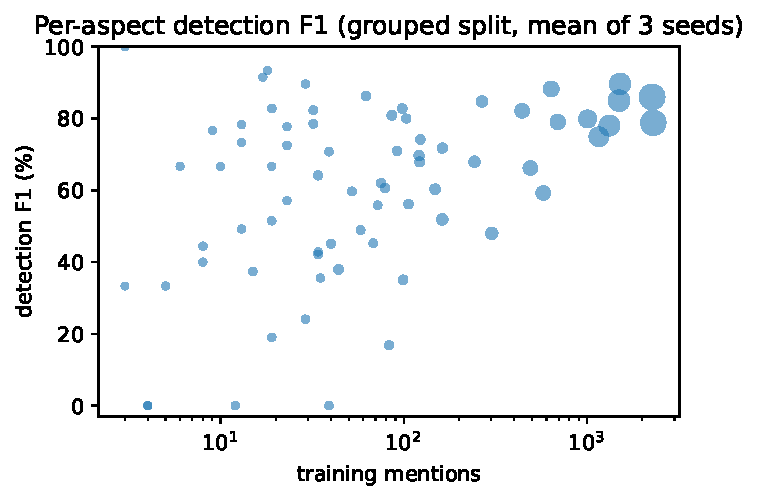
\includegraphics[width=0.9\columnwidth]{figures/final_aspect_f1_vs_freq.pdf}
\caption{Per-aspect detection F1 vs.\ training mentions (grouped split, mean of three seeds).}
\label{fig:freq}
\end{figure}

% =========================================================================
\section{Conclusion}
Writing all candidate aspect names into a fine-tuned encoder and reading a bidirectional Gated
DeltaNet memory with the pooled names gives large and significant gains for ABSA of code-mixed Bangla
reviews, most of all for unseen categories and aspect names. The delta-rule memory contributes where
an additive xLSTM memory does not: on unseen and rare aspect names.

\section*{Limitations}
Our reproduction of the official split may differ from the original. Fine-tuned XLM-R and some ablations
have one or two seeds, and XLM-R was fine-tuned with frozen word embeddings to fit into 4\,GB (as was our
model). The bootstrap captures test-set sampling, not training variance; the memory effects are 1--2
points. The zero-shot split has four categories and 18 unseen names. On BABSA, our improvement over
fine-tuned BanglaBERT is not significant. Both datasets come from Bangladesh.

\section*{Ethics Statement}
Both datasets are public (EComReviews-BD CC BY 4.0, BABSA CC BY-NC-SA 4.0, used for non-commercial
research). Systems that miss negative aspects more often could favour sellers; deployments should be
audited. An AI assistant helped write code and draft text; the authors verified all code, numbers and
citations.

\bibliography{references}

\end{document}
